\documentclass[
a4paper,
%13pt,
fontsize=13pt
]{report}

\usepackage[T2A]{fontenc}
\usepackage[utf8]{inputenc}
\usepackage[russian]{babel}
\usepackage{setspace}
\usepackage[fontsize=14pt]{scrextend}
\usepackage[table,xcdraw]{xcolor}
%\usepackage[hscale=0.78,vscale=0.8]{geometry} % margins
\usepackage[
left=30mm,
right=10mm,
bottom=20mm,
top=15mm
]{geometry}

\usepackage{sectsty}
\chaptertitlefont{\LARGE}

%\titlespacing*{\chapter}{0pt}{3.5ex plus 1ex minus .2ex}{2.3ex plus .2ex}
\usepackage{titlesec}
\titleformat{\chapter}{\normalfont\LARGE\bfseries}{\thechapter}{1em}{}




\usepackage{amsmath} 
\usepackage{listings}
\usepackage{pdflscape}
\usepackage{graphicx}
\usepackage{subfig}
\usepackage[hidelinks]{hyperref}
%\usepackage[colorlinks = true, linkcolor=black, urlcolor=black]{hyperref}
\usepackage{amssymb}
\usepackage[numbers]{natbib}
\usepackage{enumerate}
%\usepackage{color}

\usepackage{verbatim}
\usepackage{minted}

%\renewcommand{\thefigure}{\arabic{section}.\arabic{figure}}
%\renewcommand{\thetable}{\arabic{section}.\arabic{table}}

\begin{document}
\onehalfspacing
\begin{titlepage}
  
  \begin{center}
    \textbf{% Министерство науки и высшего образования \\
      % Российской Федерации\\
      Федеральное государственное автономное образовательное
      учреждение высшего образования\\
      <<Российский университет дружбы народов имени Патриса Лумумбы>>}\\[5mm]
    Факультет физико-математических и естественных наук \\[2mm]
    Кафедра прикладной информатики и теории вероятностей

    \vfill

    
    
    \vfill

    Направление: 09.03.03 Прикладная информатика

    \vfill

    ОТЧЕТ

    \bigskip
    
    о прохождении учебной практики

    Научно-исследовательская работа
    
    (получение первичных навыков научно-исследовательской работы)

    \medskip
    
    Место прохождения практики: отдел технической поддержки
    пользователей (департамент технологических и информационных
    ресурсов) РУДН и научные центры института прикладной математики
    и телекоммуникаций
   
  \end{center}

\vfill

  \begin{minipage}{.45\textwidth}
    ФИО: Саргсян Арам Грачьяевич\\
    Курс, группа 4, НПИбд-02-20\\
    Студенческий билет № 1032201740 \\ \\
    Руководители практики: \\
    от РУДН к.ф.-м.н. Е.Г. Медведева \\ \\
    
    Научный руководитель: \\
    к.ф.-м.н., доц. А.В. Королькова \\ \\

    Руководитель от организации:\\
    д.т.н., проф. К.Е. Самуйлов
    
    % Выполнил: \\ [2mm]
    % студент группы НПИ-02-20\\[2mm]
    % \underline{\hspace{3cm}} Саргсян Арам Грачьяевич\\
    % (студенческий билет № 1032201740) \\[2mm] \\
    % ``\underline{\hspace{1cm}}''\underline{\hspace{3cm}}20\underline{\hspace{1cm}}г.
  \end{minipage}%
  \hfill
  
   
\vfill
Оценка \underline{\hspace{3cm}}

\centering
г. Москва

\
\centering
2023 г.
\end{titlepage}

%\newpage
\setcounter{page}{2}
\tableofcontents
\newpage
%\chapter*{Список используемых сокращений}
\addcontentsline{toc}{chapter}{Список используемых сокращений}

\mbox{}

RED --- Random Early Detection

TCP --- Transmission control protocol

NS  --- Network Simulator

NAM --- Network animator



\chapter*{Введение}
\addcontentsline{toc}{chapter}{Введение}

Согласно программе учебной практики по направлению 09.03.03
«Прикладная информатика» целями практики являются:
\begin{itemize}
\item формирование навыков использования современных научных методов
  для решения научных и практических задач;
\item формирование универсальных, общепрофессиональных и
  профессиональных компетенций в соответствии с ОС ВО РУДН;
\item формирование навыков проведения исследовательской работы;
\item формирование навыков работы с источниками данных;
\item знакомство с принципами функционирования и изучение методов
  разработки и анализа моделей функционирования сложных систем, их
  фрагментов и отдельных элементов;
\item применение методов для анализа и расчёта показателей
  функционирования сложных систем, их фрагментов и отдельных
  элементов.
\end{itemize}

Также опредены задачи практики:
\begin{itemize}
\item изучение специфики функционирования и соответствующих методов
  анализа сложных систем;
\item формирование навыков решения конкретных научно-практических
  задач самостоятельно или в научном коллективе;
\item формирование навыков проведения исследовательской работы и
  получении научных и прикладных результатов;
\item изучение принципов и методов построения моделей сложных систем
  (в том числе технических систем, сетей и систем телекоммуникаций);
\item изучение принципов и методов анализа поведения параметров
  моделей сложных систем (в том числе программных и технических
  систем, сетей и систем телекоммуникаций, и т.п.);
\item приобретение практических навыков в области изучения научной
  литературы и (или) научно-исследовательских проектов в соответсвии с
  будущим профилем профессиональной области.
\end{itemize}


Для достижении вышеупомянутых целей и задач в рамках учебной практики
по теме <<Моделирования алгоритма управления очередями RED в средстве
моделирования Mininet>> мною было выполнено следующее:
\begin{itemize}
\item рассмотрены основные методы имитационного, аналитического и
  натурного моделирования сетей;
\item исследована специфика моделирования различных сетей c помощью
  программы Mininet;
\item проведен сравнительный анализ результатов натурного0
  моделирования сети (построены и проанализированы графики размера
  TCP-окна, длины очереди и средней взвешенной длины очереди) при
  различных модификациях алгоритма RED, разных пороговых значений и
  типов TCP.
\end{itemize}

%\newpage
\chapter{Методы и материалы}

В этом разделе представим краткий обзор средств моделирования сетей
передачи данных.

\section{NS-2}
NS-2 (Network simaulator 2) — это программное средство моделирования
сетей, использующееся для исследования и анализа поведения
компьютерных сетей.  Запуск имитационной модели в данной среде
позволяет анализировать различные протоколы и алгоритмы сетевой связи.

NS-2 разработан на языке программирования С++ и TCL, что обеспечивает
гибкость и расширяемость средства моделирования.  NS-2 содержит
библиотеку классов, которые представляют различные элементы сети,
такие как узлы, маршрутизаторы, каналы связи и протоколы передачи
данных. Для создания модели сети определяются характеристики и
параметры каждого элемента сети: пропускная способность канала,
задержки, вероятность потери пакетов и другие. После завершения
симуляции NS-2 предоставляет мощные инструменты анализа результатов,
включая возможность визуализации данных посредством программы NAM
(Network animator), статистический анализ и сравнение результатов
экспериментов, что позволяет изучать и оценивать производительность
различных протоколов и алгоритмов в различных сценариях
сети ~\citep{{NS2-1}, {NS2-2}}.

\section{Mininet}

Mininet — это симулятор сетевых топологий на основе виртуаилизации,
который позволяет моделировать и изучать поведение сетей в
контролируемой среде, основанный на использовании виртуальных машин и
пространств имен Linux для создания изолированных сетевых
узлов. Моделирование сетевых топологий с помощью Mininet позволяет
исследовать различные сетевые протоколы, маршрутизацию, управление
трафиком и т.д. Возможности моделирования с помощью Mininet включают
создание виртуальных сетевых узлов, конфигурирование топологий (связь
между узлами, настраивать IP-адреса, маршрутизацию), имитировать
различные условия сети, такие как задержки, потери пакетов и
пропускную способность, интеграция с контроллерами для исследования
новых протоколов и алгоритмов ~\citep{mininet}. 

Некоторые характеристики, которые указали на создание Mininet, включают в себя:

\begin{itemize}
  \item \textbf{Гибкость:} новые топологии и функции могут быть настроены в программном обеспечении с использованием языков программирования и распространенных операционных систем.
  
  \item \textbf{Применимость:} правильно реализованные прототипы должны быть применимы в реальных сетях на базе оборудования без изменений в исходных кодах.
  
  \item \textbf{Интерактивность:} управление и запуск симулированной сети должны происходить в режиме реального времени, как если бы это происходило в реальных сетях.
  
  \item \textbf{Масштабируемость:} среда прототипирования должна масштабироваться до крупных сетей с сотнями или тысячами коммутаторов на одном компьютере.
  
  \item \textbf{Реализм:} поведение прототипа должно соответствовать реальному поведению с высокой степенью уверенности, чтобы приложения и протоколы могли использоваться без изменений в коде.
  
  \item \textbf{Возможность совместного использования:} созданные прототипы должны быть легко совместно используемыми с другими сотрудниками, которые могут выполнять и модифицировать эксперименты.
\end{itemize}

\subsection{Iperf3}

iPerf3 представляет собой кроссплатформенное клиент-серверное приложение с открытым исходным кодом,
которое можно использовать для измерения пропускной способности между
двумя конечными устройствами. iPerf3 может работать с транспортными протоколами TCP, UDP и SCTP:

TCP и SCTP:

\begin{itemize}

\item измерение пропускной способности
\item возможность задать размер MSS/MTU
\item отслеживание размера окна перегрузки TCP (CWnd)

\end{itemize}

UDP:
\begin{itemize}
\item измерение пропускной способности
\item измерение потери пакетов
\item измерение колебания задержки (jitter)
\item поддержка групповой рассылки пакетов (multicast).
\end{itemize}

\subsection{Netem}

NETEM —  это сетевой эмулятор Linux, используемый для тестирования производительности реальных клиент-серверных приложений в виртуальной сети. 
Модуль управляется при помощи команды tc из пакета iproute2. 
NETEM позволяет пользователю задать ряд параметров сети, такие как задержка, дрожание задержки (jitter), уровень потери пакетов, дублирование и изменение
порядка пакетов. Данный эмулятор состоит из двух частей: модуля ядра для организации очередей и утилиты командной строки для его настройки. Между
протоколом IP и сетевым устройством создаётся очередь с дисциплиной обслуживания. Дисциплина обслуживания очереди реализуется как объект с двумя
интерфейсами. Один интерфейс ставит пакеты в очередь для отправки, а другой
интерфейс отправляет пакеты на сетевое устройство. На основе дисциплины
обслуживания очередей принимается решение о том, какие пакеты отправлять,
какие пакеты задерживать и какие пакеты отбрасывать.
Дисциплины обработки очередей можно разделить на бесклассовые и классовые. Бесклассовые дисциплины, используемые по умолчанию в общем, получают данные, переупорядочивают,
вносят задержку или уничтожают их. Наиболее распространённой бесклассовой дисциплиной является FIFO
(первым пришёл, первым обслужен).
Классовые дисциплины широко используются в случаях, когда тот или иной
вид трафика необходимо обрабатывать по разному. Примером классовой дисциплины может служить CBQ — Class Based Queueing (дисциплина обработки
очередей на основе классов). Классы трафика организованы в дерево— у каждого
класса есть не более одного родителя; класс может иметь множество потомков.
Классы, которые не имеют родителей, называются корневыми. Классы, которые
не имеют потомков, называются классами-ветками.
Модуль управляется при помощи команды tc из пакета iproute2. 



\section{Cisco Packet Tracer}

Packet Tracer — это программное средство, предоставляемое компанией
Cisco Systems, позволяющей смоделировать, конфигурировать и отлаживать
сетевые сценарии, широко используемое в области сетевых
технологий. Данное программное обеспечение предоставляет виртуальную
среду, которое позволяет создавать сетевые топологии и настраивать
устройства Cisco: маршрутизаторы, коммутаторы и т.д. Графический
интерфейс позволяет соединять устройства, устанавливать параметры
соединений и задавать настройки протоколов. Cisco Packet Tracer
позволяет имитировать передачу данных в сети. Пользователи могут
выполнять различные тесты связи, проводить диагностику и мониторинг
сетевых устройств, а также создавать и анализировать журналы событий.

\section{GNS-3}

GNS-3 — это программное средство моделирования сетей, позволяющий
создавать виртуальные сети, состоящие из реальных или виртуальных
устройств, и анализировать их поведение. GNS-3 разработан на языке
программирования Python и основан на эмуляторе динамических узлов
Dynamips, который позволяет запускать реальные образы операционных
систем. В отличие от Packet Tracer, GNS-3 позволяет смоделировать не
только устройства Cisco, но и другие устройства, например, Juniper,
Palo, Alto и другие, что позволяет смоделировать различные типы сетей,
включая центры обработки данных и облачные инфраструктуры. Одной из
главных особенностей GNS-3 является интеграция с виртуальными
машинами, что расширяет возможности моделирования. Появляется
возможность создавать сетевые сценарии, в которых виртуальные машины
выполняют реальные функции, такие как серверы, клиенты, точки доступа
Wi-Fi и т.д. Это позволяет проводить натурное моделирование и
получить более реалистичные результаты в рамках виртуальной среды.







%\chapter{RANDOM EARLY DETECTION}

\section{RED}


Random Early Detection (RED) — это механизм предотвращения перегрузки
на шлюзе. Он основан на общих принципах, полезен для управления
средним размером очереди в сети, где не доверяют взаимодействию между
протоколами передачи данных. В отличие от Droptail, который работает
таким образом, что когда очередь заполняется, новые пакеты,
поступающие в очередь, начинают теряться, алгоритм RED учитывает
потоки трафика в сети и стремится предоставить равную пропускную
способность для каждого соединения, что позволяет избежать перегрузки
сети и улучшить качество обслуживания. В оригинальном RED
маршрутизатор вычисляет усредненный по времени средний размер очереди
с использованием фильтра нижних частот (экспоненциально взвешенное
скользящее среднее) или сглаживания по длине выборки очередей, средний
размер очереди сравнивается с двумя пороговыми значениями: минимальным
порогом и максимальным. Когда средний размер очереди меньше
минимального порога, пакеты не отбрасываются, когда средний размер
очереди превышает максимальный порог, отбрасывается все поступающие
пакеты. Если размер средней очереди находится между минимальным и
максимальным порогом, пакеты отбрасываются с вероятностью $p$, которая
линейно увеличивается до тех пор, пока средняя очередь не достигнет
максимального порога. Подробно алгоритм описан в~\citep{{RED1},{RED2}}.
 
Вероятность $p_{b}$ маркировки на отбрасывание пакетов представляет
собой функцию, линейно зависящую от $\hat{q}$ (средневзвешенное
скользящее среднее), минимального $q_{\min}$ и максимального
$q_{\max}$ пороговых значений и параметра $p_{\max}$, определяющего
часть отбрасываемых пакетов при достижении средним размером очереди
значения $q_{\max}$ и вычисляется следующим образом(\ref{red}):

\begin{equation}
\label{red}
p_{b} = \begin{cases}
        0, &  \ 0 < \hat{q} \leqslant q_{\min},
        \\
        \frac{\hat{q} - q_{\min}}{q_{\max} - q_{\min}} p_{\max}, & \ q_{\min} < \hat{q} \leqslant q_{\max}, 
        \\
        1, &  \ \hat{q} > q_{\max}.
\end{cases}                                     
\end{equation}

График функции вероятности потери пакета в зависимости от среднего
размера очереди представлен на рис.~\ref{fig:2.1}.

\begin{figure}[!h]
  \centering
  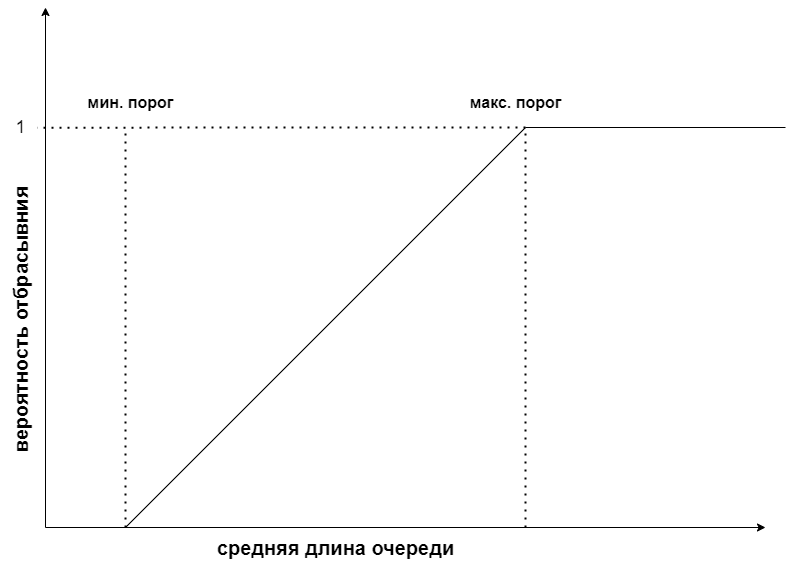
\includegraphics[width=0.7\linewidth]{image/red.png}
  \caption{Классический RED}
  \label{fig:2.1}
\end{figure}


В NS-2 файлы, связанные с RED, прописаны в каталоге
\verb|ns-2.35/queue|, там представлены также другие реализации
очередей (среди них DropTail, BLUE и т.д.). Следует уделить внимание
двум файлам: \verb|red.cc| (исходники), и \verb|red.h| (заголовочный
файл). Вероятность отбрасывания пакета прописана в функции 
\verb|double REDQueue::calculate_p_ne файла red.cc|

Для реализации в NS-2 необходимо указать в качестве очередей между соединениями
RED, и при настройке очереди указать минимальные и максимальные пороговые значения 
\verb|(thresh_ и maxthresh_)|, величина, обратное параметру максимального сброса\verb|(linterm_)|, 
а также указать параметр \verb|gentle_| false.


\section{GRED} 

GRED (Gentle Random Early Detection, мягкое/аккуратное произвольное
раннее обнаружение)~--- алгоритм активного управления очередью,
является расширением RED. Стандартный алгоритм увеличивает
вероятность отбрасывания с 0.05 до 0.5, когда средняя длина очереди
увеличивается от минимального до максимального порогового значения, но
при превышении максимального порога вероятность возрастает напрямую с
0.5 до 1.  Этот внезапный скачок нормализуется модификацией Gentle
RED, который расширяет RED тем, что добавляет дополнительное
максимальное пороговое значние, которое равно $2q_{\max}$, тем самым
<<сглаживая>> кривую~\citep{GRED}. Однако, например, задача минимального порога в данной модификации не меняется, 
и увеличение лишь максимального порога для отбрасывания всех пакетов делает GRED лишь частным случаем классического алгоритма. 
Данная модификация в NS-2 является основной, так как переменная \verb|gentle_| по умолчанию 
является истинной. 

Вероятность сброса определяется следующим образом (\ref{gred}):

\begin{equation}
\label{gred}
p_{b} =\begin{cases}
        0, &  \  0 < \hat{q} \leqslant q_{\min}, 
        \\
        \frac{\hat{q} - q_{\min}}{q_{\max} - q_{\min}} p_{\max}, & \ q_{\min} \leqslant \hat{q} < q_{\max}, 
        \\
        \frac{\hat{q} - q_{\min}}{q_{\max}}(1-p_{\max}) - p_{\max}, & \ q_{\max} \leqslant \hat{q} < 2q_{\max}, 
        \\
        1, &  \ \hat{q} \geqslant  q_{\max}.
\end{cases}
\end{equation}

График функции вероятности потери пакета в зависимости от среднего
размера очереди выглядит следующим образом (рис.~\ref{fig:2.2}):

\begin{figure}[!h]
  \centering
  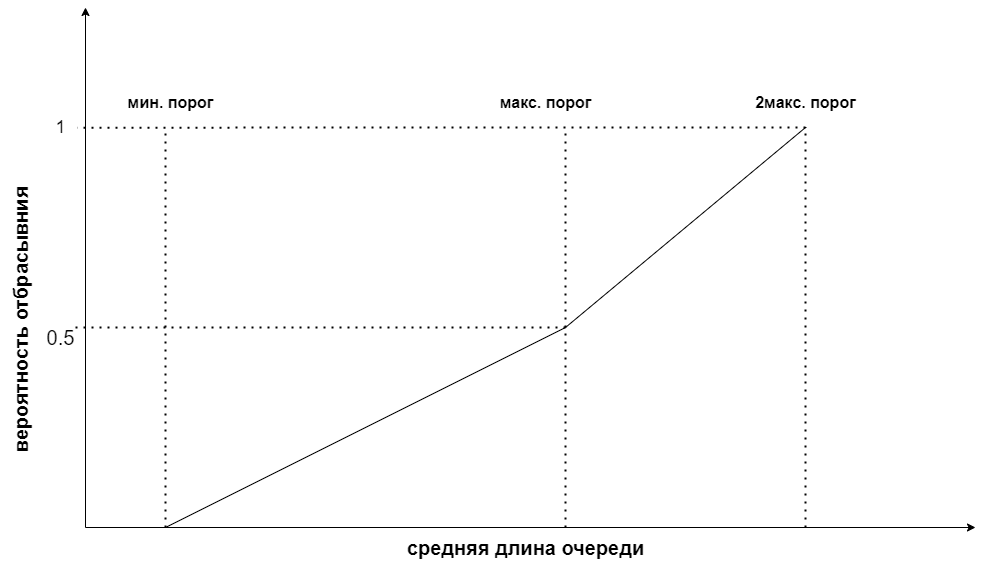
\includegraphics[width=0.7\linewidth]{image/gred.png}
  \caption{Gentle RED}
  \label{fig:2.2}
\end{figure}


\section{WRED}

WRED (Weighted random early detection --- взвешенное произвольное раннее
обнаружение)~--- это алгоритм активного управления очередью, является
расширением RED~\citep{WRED}.

Взвешенный алгоритм произвольного раннего обнаружения предоставляет
различные уровни обслуживания пакетов в зависимости от вероятности их
отбрасывания и обеспечивает избирательную установку параметров
механизма RED на основании типа трафика (рис.~\ref{fig:2.3}).

\begin{figure}[!h]
  \centering
  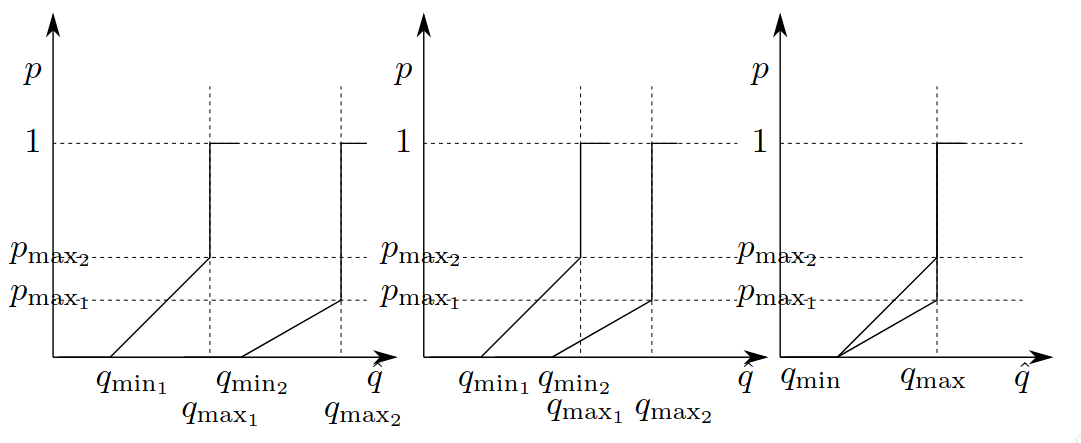
\includegraphics[width=0.7\linewidth]{image/wred.png}
  \caption{Weighted RED}
  \label{fig:2.3}
\end{figure}

\section{NLRED}

Nonlinear RED~--- это модификация классического алгоритма RED, в
котором используется нелинейная функция для определения
вероятности отбрасывания пакетов. Nonlinear RED предназначен для более точной адаптации к изменениям трафика и динамике сети. 
Он способен эффективно реагировать на изменения величины очереди и адаптироваться к различным условиям сети. 
Это позволяет более гибко управлять задержкой пакетов и предотвращать перегрузки в сети, 
что делает Nonlinear RED более эффективным по сравнению с классическим алгоритмом RED.~\citep{NLRED1,NLRED2}.   


Вероятность $p_{b}$ маркировки на
отбрасывание пакетов вычисляется следующим способом (\ref{nlred}):

\begin{equation}
\label{nlred}
p_{b} = \begin{cases}
        0, &  \ 0 < \hat{q} \leqslant q_{\min},
        \\
        1.5({\frac{\hat{q} - q_{\min}}{q_{\max} - q_{\min}})^2} {p_{\max}}, & \ q_{\min} < \hat{q} \leqslant q_{\max},
        \\
        1, &  \ \hat{q} > q_{\max}.
\end{cases}
\end{equation}

График функции вероятности потери пакета в зависимости от среднего
размера очереди представлен на  рис.~\ref{fig:2.4}.

\begin{figure}[!h]
  \centering
  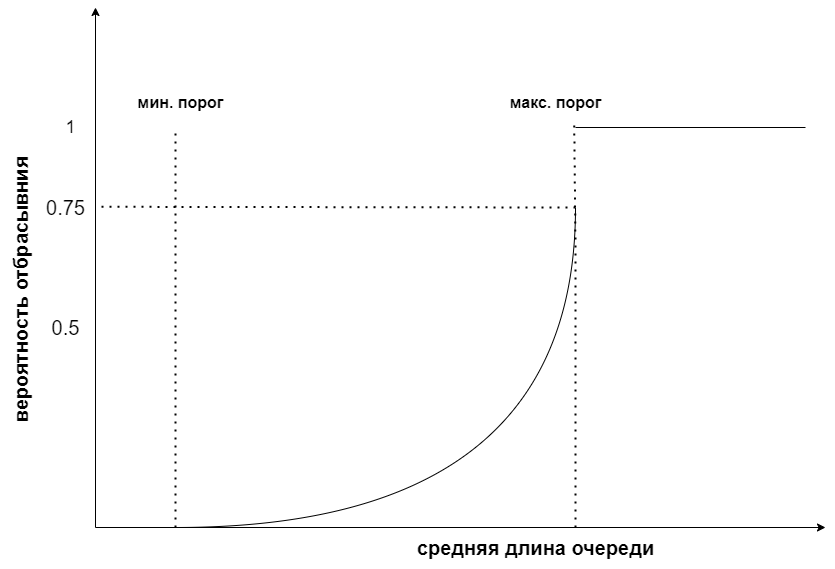
\includegraphics[width=0.7\linewidth]{image/nlred.png}
  \caption{NonLinear RED}
  \label{fig:2.4}
\end{figure}

По умолчанию NLRED не реализован в NS-2. Для её добавления я использовал патч для данной модификации, созданный Mohit
  P. Tahiliani для версии 2.34, совместимой также для версии 2.35. 
  
\begin{enumerate}
\item Установил к себе на машину патч \verb|NLRED.patch| от 
\item Отредактировал файл, заменив везде номер версии на 2.35 и переместил в каталог \verb|ns-allinone|.
\item Дополнил файлы \verb|queue/red.cc|, \verb|queue/red.h|, \verb|tcl/ns-default.tcl| строками из патча, .
\item Переустановил программу.
\item В настройке очереди сети указал значение переменной \verb|nonlinear_ 1|.
\end{enumerate}
 
 
\section{HRED} 
 
HRED(Hyperbola random early detection) ~---это модификация классического RED с нилейно возрастающей функцией отбрасывания пакетов в сети.
HRED менее чувствителен к настройкам параметров, чем другие схемы. При заданном значении $q_{\max}$ HRED ведет себя похожим образом и не сильно зависит от других параметров.
HRED может достичь более высокого использования сети. HRED обеспечивает предсказуемую задержку в очереди сети. HRED сохраняет способность контролировать кратковременную перегрузку путем поглощения пакетных потоков, так как он все еще использует алгоритм подсчета среднего размера очереди и поддерживает неполную очередь. Размер очереди может быть задан и зависит от требований. HRED прост в реализации и легко внедряется на маршрутизаторах, так как зменяется только профиль отбрасывания по сравнению с классическим алгоритмом RED~\citep{HRED}. По умолчанию модификация не реализована в NS-2, для её реализации дополнил фунцию \verb|double REDQueue::calculate_p_ne файла red.cc|, а в программе очереди указал значение переменной \verb|hyperbola_ 1|.
 
Вероятность $p_{b}$ маркировки на
отбрасывание пакетов вычисляется следующим способом (\ref{nlred}):

\begin{equation}
\label{nlred}
p_{b} = \begin{cases}
        0, &  \ 0 < \hat{q} \leqslant q_{\min},
        \\
        1.5({\frac{\hat{q} - q_{\min}}{q_{\max} - q_{\min}})^{-1}} {p_{\max}}, & \ q_{\min} < \hat{q} \leqslant q_{\max},
        \\
        1, &  \ \hat{q} > q_{\max}.
\end{cases}
\end{equation}



\section{TRED}

TRED(Three-section random early detection) ~--- это разновидность алгоритма RED, основанный на Nonlinear RED, которая направлена на решение проблем недостаточного использования пропускной способности и больших задержек, возникающих при низкой и высокой нагрузке в RED. 
Средняя длина очереди TRED между двумя пороговыми значениями разделена на три равные секции, и вероятность отбрасывания пакетов для каждой секции устанавливается по-разному, чтобы адаптироваться к различным трафиковым нагрузкам. С использованием симуляции в среде NS2, TRED эффективно устраняет недостатки RED, увеличивая пропускную способность при низкой нагрузке и снижая задержку при высокой нагрузке. TRED улучшает способность регулировать сетевую перегрузку, повышая использование ресурсов сети и стабильность схемы. В дальнейших исследованиях мы заинтересованы в изучении TRED с явным уведомлением о перегрузке (ECN), поскольку множество исследований показало, что AQM с ECN работает более эффективно, чем без ECN.~\citep{TRED}. По умолчанию модификация не реализована в NS-2, для её реализации дополнил фунцию \verb|double REDQueue::calculate_p_ne файла red.cc|, а в программе очереди указал значение переменной \verb|three_sections_ 1|. 

Вероятность $p_{b}$ маркировки на отбрасывание приведена в (\ref{TRED}), где $ \delta = (q_{max} - q_{min})/3 $.

\begin{equation}
\label{TRED}
p_{b} = \begin{cases}
        0, &  \ 0 \leqslant \hat{q} < q_{\min},
        \\
        9({\frac{\hat{q} - q_{\min}}{q_{\max} - q_{\min}})^3} {p_{\max}}, & \ q_{\min} \leqslant  \hat{q} < q_{\min + \delta},
        \\
        (\frac{\hat{q} - q_{\min}}{q_{\max} - q_{\min}}) {p_{\max}}, & \ q_{\min} + \delta \leqslant \hat{q} < q_{\min + 2\delta},
        \\
        9({\frac{\hat{q} - q_{\min}}{q_{\max} - q_{\min}})^3} {p_{\max}} + {p_{\max}}, & \ q_{\min} +2\delta \leqslant  \hat{q} < q_{\max},
        \\
        1, &  \ \hat{q} \geqslant q_{\max}.
\end{cases}
\end{equation} 

\section{RED-QL}

RED-QL(Random early detection-quadratic linear) ~---модификация алгоритма RED, также является разновидностью алгоритма с нелинейно возрастающей функцией. RED-QL имеет квадратично-линейную форму и определяется на основе параметров, которые могут быть настроены для определенных требований сети\citep{REDQL} По умолчанию модификация не реализована в NS-2, для её реализации дополнил фунцию \verb|double REDQueue::calculate_p_ne файла red.cc|, а в программе очереди указал значение переменной \verb|quadratic_linear_ 1|. . 

Вероятность $p_{b}$ маркировки на отбрасывание приведена в (\ref{RED-QL}), где $ Target = 2(q_{max} + q_{min})/3 - q_{min} $.

\begin{equation}
\label{RED-QL}
p_{b} = \begin{cases}
        0, &  \ 0 \leqslant \hat{q} < q_{\min},
        \\
        9({\frac{\hat{q} - q_{min}}{2(q_{\max} - 2q_{\min}})^2} {p_{\max}}, &  q_{\min} \leqslant  \hat{q} < {Target},
        \\
        p_{max} + 3(1-p_{max}) (\frac{\hat{q} - Target}{q_{\max} + q_{\min}}), & {Target} \leqslant  \hat{q} < q_{max},
        \\
        1, &  \ \hat{q} \geqslant q_{max}.
\end{cases}
\end{equation}

\section{SmRED}

SmRED(Smart random early detection) ~--- модификация RED, в которой
вероятность отбрасывания пакетов регулируется в зависимости от нагрузки трафика для достижения оптимальной сквозной производительности.
Кроме того, переход с RED на SmRED в реальной сети требует очень мало работы из-за своей простоты. SmRED эффективно устраняет недостатки
RED, увеличивает пропускную способность при низкой нагрузке и уменьшает задержку при высокой нагрузке ~\citep{SmRED}. По умолчанию модификация не реализована в NS-2, для её реализации дополнил фунцию \verb|double REDQueue::calculate_p_ne файла red.cc|, а в программе очереди указал значение переменной \verb|smart_ 1|. 

Вероятность $p_{b}$ маркировки на отбрасывание приведена в (\ref{SmRED}), где $ Target = (q_{max} - q_{min})/2 + q_{min} $.

\begin{equation}
\label{SmRED}
p_{b} = \begin{cases}
        0, &  \ 0 \leqslant \hat{q} < q_{\min},
        \\
        ({\frac{\hat{q} - q_{min}}{q_{\max} - q_{\min}})^2} {p_{\max}}, &  q_{\min} \leqslant  \hat{q} < {Target},
        \\
        \sqrt{{\frac{\hat{q} - q_{min}}{q_{\max} - q_{\min}}}} {p_{\max}}, & {Target} \leqslant  \hat{q} < q_{max},
        \\
        1, &  \ \hat{q} \geqslant q_{max}.
\end{cases}
\end{equation}


\section{DS-RED}

Алгоритм DS-RED(Double slope random early detection)~--- это ещё одна модификация RED, в котором вводится дополнительное пороговое значение $q_{mid}$ между минимальным $q_{min}$ и максимальным
REDФункция сброса описывается двумя линейными сегментами с углами наклона $\alpha $ и $\beta $ соответственно, регулируемыми
задаваемым селектором режимов $\gamma$ ~\citep{DSRED}.  По умолчанию модификация не реализована в NS-2, для её реализации дополнил фунцию \verb|double REDQueue::calculate_p_ne файла red.cc|, а в программе очереди указал значение переменной \verb|double_slope_ 1|. 

Функция вероятности сброса пакетов в алгоритме DSRED показана в (\ref{dsred})

\begin{equation}
\label{dsred}
p_{b} =\begin{cases}
        0, &  \  0 < \hat{q} \leqslant q_{min}, 
        \\
        \alpha{\hat{q} - q_{min}}, & \ q_{min} \leqslant \hat{q} < q_{mid}, 
        \\
        1 - \gamma + \beta{\hat{q} - q_{mid}}, & \ q_{mid} \leqslant \hat{q} < q_{max}, 
        \\
        1, &  \ \hat{q} \geqslant  q_{max}.
\end{cases}
\end{equation}

где $\alpha = (\frac{2(1 - \gamma)}{\hat{q} - q_{\min}})$, а $\beta = (\frac{2\gamma}{\hat{q} - q_{min}})$

\section{ARED}

В алгоритме Adaptive RED (ARED) функция сброса модифицируется
посредством изменения по принципу AIMD, заключающейся в том, что
увеличение некоторой величины производится путём сложения с некоторым
параметром, у уменьшение~--- путём умножения на
параметр ~\citep{ARED}. Для её реализации в NS-2 необходимо указать в
настройке очереди \verb|set adaptive_ 1|,.

Алгоритм ARED функционирует следующим образом (\ref{ad1}),
(\ref{ad2}). Для каждого интервала \verb|interval| (параметр) в
секундах, если $\hat{q}$ больше целевой (желаемой) $\hat{q_t}$ и
$p_{\max} \leqslant 0,5$, то $p_{\max}$ увеличивается на некоторую
величину $\alpha$; в противном случае, если $\hat{q}$ меньше целевой
$\hat{q_t}$ и $p_{\max}\geqslant 0,01$, то $p_{\max}$ уменьшается в
$\beta$ раз, $\alpha$ и $\beta$ задаются командами \verb|set alpha_| и \verb|set beta_|:

\begin{equation}
\label{ad1}
p_{\max} = \left\{
  \begin{aligned}
    & p_{\max}+\alpha, \ \hat{q}>\hat{q_{t}}, \ p_{\max} \leqslant 0,5, \\
    & \beta p_{\max}, \ \hat{q}<\hat{q_{t}}, \ p_{\max} \geqslant 0,01, 
  \end{aligned}
\right.
\end{equation}

\begin{equation}
\label{ad2}
q_{\min}+0,4(q_{\max}-q_{\min}) < \hat{q_t} < q_{\min}+0,6\left(q_{\max}-q_{\min}\right).
\end{equation}

Основные особенности: 
\begin{itemize}
\item автоматическая установка минимального порога $q_{\min}$. Он
  устанавливается в зависимости от пропускной способности канала $C$ и
  задержки целевой очереди, $q_{max}$ приравнивается к $3q_{min}$;
\item автоматическая настройка $w_{q}$. Он устанавливается в
  зависимости от пропускной способности канала $C$;
\item адаптивная настройка $p_{\max}$. Он адаптирован в соответствии с
  текущей средней длиной очереди;
\item рекомендованными значениями параметров являются $\alpha < 0.25 $ и $\beta > 0.83 $.
\end{itemize}


\section{RARED}

Алгоритм Refined ARED является модификацией
ARED и предлагает более активно изменять вероятность сброса $p_{\max}$,
чтобы иметь возможность быстрой адаптации к изменяющейся
экспоненциально взвешенной скользящей средней длине очереди $\hat{q}$ ~\citep{RARED}.

Функции изменения параметра $p_{\max}$ представлена ниже(\ref{rf1}), (\ref{rf2}):

\begin{equation}
\label{rf1}
p_{max} = \left\{
  \begin{aligned}
& p_{\max}+\alpha, \quad  \hat{q}>\hat{q_{t}}, \quad p_{max} \leqslant 0,5, \\
& \beta p_{\max}, \quad \hat{q}\leqslant\hat{q_{t}}, \quad p_{max} > 0,5,
  \end{aligned}
\right.
\end{equation}

\begin{equation}
\label{rf2}
\left\{
  \begin{aligned}
    & q_{\min}+0,48\left(q_{\max}-q_{\min}\right) < \hat{q_t} < q_{\min}+0,52\left(q_{\max}-q_{\min}\right), \\
    & \alpha=\left(0,25\frac{\hat{q}-\hat{q_t}}{\hat{q_t}} \right)p_{\max}, \\ 
    & \beta=1-\left(0,17\frac{\hat{q}-\hat{q_t}}{\hat{q_t}-q_{\min}}\right).
  \end{aligned}
\right.
\end{equation}


По умолчанию Refined ARED не реализован в NS-2. Для его добавления я
проделал следующие шаги:

\begin{enumerate}
\item Установил к себе на машину патч \verb|RARED.patch| от 
\item Отредактировал файл, заменив везде номер версии на 2.35 и переместил в каталог \verb|ns-allinone|.
\item Дополнил файлы \verb|queue/red.cc|, \verb|queue/red.h|, \verb|tcl/ns-default.tcl| строками из патча.
\item Переустановил программу.
\item В настройке очереди указал значение \verb|adaptive_ 1| и 
\verb|refined_adaptive_ 1|.
\end{enumerate}
 
 
\section{Powared}

Powared является модификацией алгоритма ARED ~\citep{Powared}. В данной модификации величина $p_{max}$ максимального сброса считается следующим образом(\ref{powared}). Алгоритм POWARED более агрессивно реагирует на изменение cредней очереди, чем ARED. Данная модификация не реализована в NS-2, для её моделирования я в файл red.cc добавил функцию \verb|void REDQueue::updateMaxP_powared|, а в настройке очереди сети указал значение переменных \verb|adaptive_ 1| и \verb|powared_ 1|. 
Параметры модификации задаются с помощью переменных \verb|pwk_, pwb_|.

\begin{equation}
\label{powared}
p_{max} =\begin{cases}
        p_{max}-\delta_1, &  \  q_{\min} \leqslant \hat{q} < q_{mid}, 
        \\
        p_{max}+\delta_2, & \ q_{mid} < \hat{q}  \leqslant q_{max}, 
        \\
        p_{max}, &  \ \hat{q} =  q_{mid},
\end{cases}
\end{equation}

где $q_{mid} = 0.5(q_{min} + q_{max})$, 
$\delta_1 = |\frac{((\hat{q} - q_{mid})}{(\beta q_{mid}))}|^K $, а $\delta_2 = |\frac{((q_{mid} - \hat{q})}{(\beta (R -q_{mid})))}|^K.$


\section{FARED}

FARED(Fast Adapting RED)~--- это алгортитм, который сохраняет целевой диапазон, указанный в алгоритме RARED, но изменяет верхнюю и нижнюю границы для $\alpha $ и $\beta$ соответственно. Алгоритм FARED обеспечивает надежную производительность в широком диапазоне сред, включая сценарии с умеренной и высокой нагрузкой на трафик~\citep{Tahiliani_2012}.
Данная модификация не требует установки каких-либо дополнительных параметров для повышения производительности. Поскольку в алгоритм FARED внесены лишь незначительные изменения по сравнению
с ARED и ReARED, он может быть развернут без каких-либо сложностей(\ref{fared1}, \ref{fared2}). Данная модификация не реализована в NS-2, для её моделирования я в файл red.cc добавил функцию \verb|void REDQueue::updateMaxP_fast_adaptive|, а в настройке очереди сети указал значение переменных \verb|adaptive_ 1| 
и \verb|fast_adaptive_ 1|. 

\begin{equation}
\label{fared1}
p_{max} = \left\{
  \begin{aligned}
& p_{\max}+\alpha, \quad  \hat{q}>\hat{q_{t}}, \quad p_{max} \leqslant 0,5, \\
& \beta p_{\max}, \quad \hat{q}\leqslant\hat{q_{t}}, \quad p_{max} > 0,5,
  \end{aligned}
\right.
\end{equation}

\begin{equation}
\label{fared2}
\left\{
  \begin{aligned}
    & q_{\min}+0,48\left(q_{\max}-q_{\min}\right) < \hat{q_t} < q_{\min}+0,52\left(q_{\max}-q_{\min}\right), \\
    & \alpha=\left(0,0412\frac{\hat{q}-\hat{q_t}}{\hat{q_t}} \right)p_{\max}, \\ 
    & \beta=1-\left(0,0385\frac{\hat{q}-\hat{q_t}}{\hat{q_t}-q_{\min}}\right).
  \end{aligned}
\right.
\end{equation}



\chapter{Результаты}

Мною был написана программа, реализующая имитационную модель сети со следующей топологией:
\begin{itemize}
\item $N=20$ TCP-источников, $N$ TCP-приёмников, двух маршрутизаторов $R1$
  и $R2$ между источниками и приёмниками ($N$ — не менее 20);
\item между TCP-источниками и первым маршрутизатором установлены
  дуплексные соединения с пропускной способностью 100 Мбит/с и
  задержкой 20 мс очередью типа DropTail;
\item между TCP-приёмниками и вторым маршрутизатором установлены
  дуплексные соединения с пропускной способностью 100 Мбит/с и
  задержкой 20 мс очередью типа DropTail;
\item между маршрутизаторами установлено симплексное соединение
  ($R1$--$R2$) с пропускной способностью 20 Мбит/с и задержкой 15 мс
  очередью типа RED, размером буфера 300 пакетов; в обратную сторону~---
  симплексное соединение ($R2$--$R1$) с пропускной способностью 15 Мбит/с и
  задержкой 20 мс очередью типа DropTail;
\item данные передаются по протоколу FTP поверх TCPReno;
\item параметры алгоритма RED: $q_{\min}=75$, $q_{\max}=150$, $q_w=0,002$, $p_{\max}=0.1$;
\item максимальный размер TCP-окна 32; размер передаваемого пакета 500
  байт; время моделирования~--- не менее 20 единиц модельного времени.
\end{itemize}

Полная реализация программы приведена в разделе \textbf{Приложения},
для вывода графиков была использована программа GNUPLOT.

Смоделировав сеть с указанными параметрами и запустив gnuplot-скрипт,
я получил следующий график (рис.~\ref{fig:3.1}).

\begin{figure}[!ht]
  \centering
  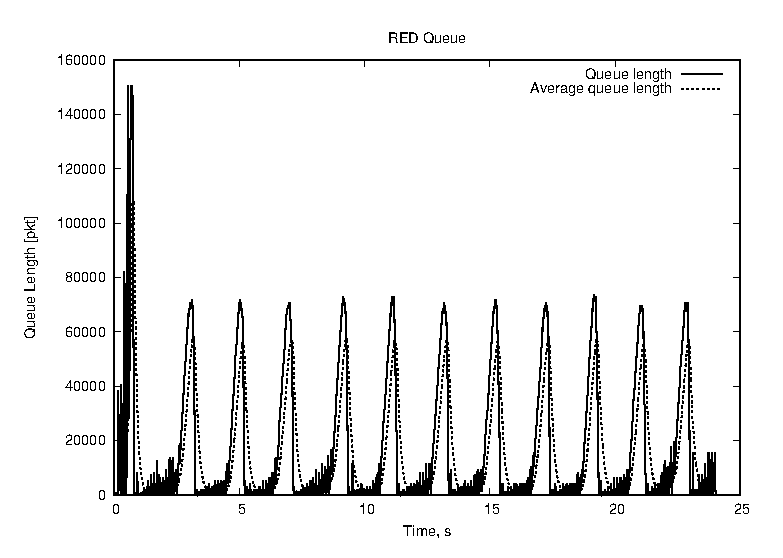
\includegraphics[width=0.6\linewidth]{image/queues_75-150_classic.eps}
  \caption{График длины очереди и средней длины очереди на
    линке (R0--R1) ($q_{\min}=75$, $q_{\max}=150$, $q_w=0.002$, $p_{\max}=0.1$,
    TCP типа TCP/Reno)}
  \label{fig:3.1}
\end{figure}

Как мы видим из первого графика, в момент времени $t=1$~c достигается
максимальные длины очереди 140000 пакетов и средней длины очереди
120000 пакетов, а при дальнейшем моделировании длина очереди
варьируются от 0 до 70000 пакетов, а средняя очередь от 0 до 60000,
наступает стационарное состояние.

Для выявления влияния пороговых значений на длину очереди смоделировал
сеть и вывел на одном графике траектории  средней длины очереди при разных
пороговых значениях и при одинаковых остальных параметрах
(рис.~\ref{fig:3.2}).

\begin{figure}[!ht]
  \centering
  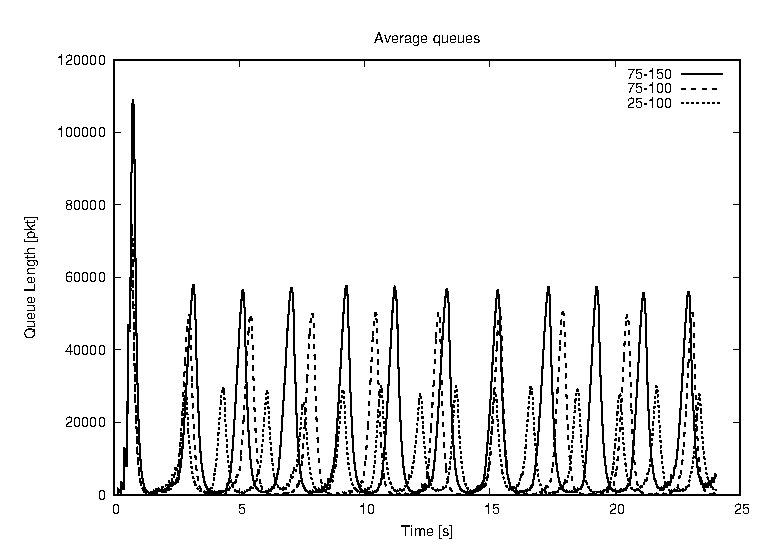
\includegraphics[width=0.7\linewidth]{image/av_queues_maxthresh.eps}
  \caption{График средней длины очереди для разных пороговых значений}
  \label{fig:3.2}
\end{figure}

Как видно из графика,
увеличение диапазона между $q_{\min}$ и $q_{\max}$ способствует
увелечению длины очереди на линке.

Для сравнений модификаций мы смоделировали сети и вывели графики очередей для всех реализованных модификаций
(рис.~\ref{fig:3.3},~\ref{fig:3.4},~\ref{fig:3.5},~\ref{fig:3.6}, ~\ref{fig:3.7}).


\begin{figure}[!ht]
  \centering
  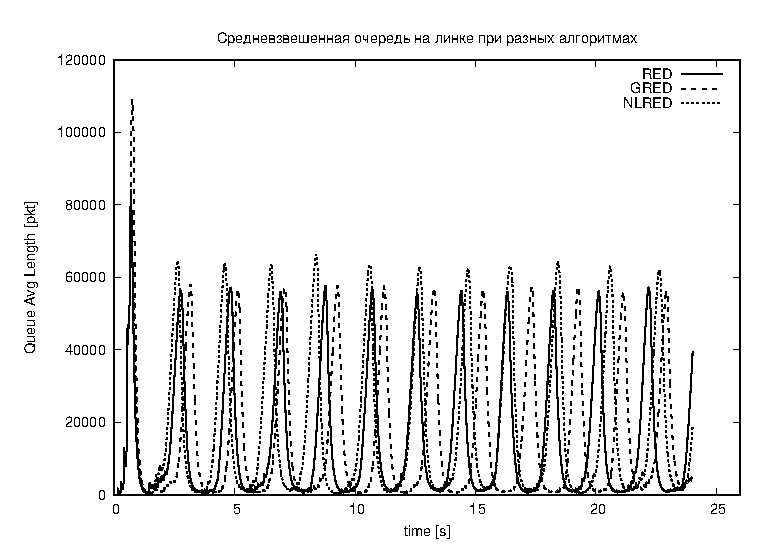
\includegraphics[width=0.7\linewidth]{image/av_queues_1GNl.eps}
  \caption{График средневзвешанной экспоненциальной очереди для RED, GRED, NLRED}
  \label{fig:3.3}
\end{figure}

Как мы видим в ~\ref{fig:3.3}, GRED и NLRED после достижения стационарного состояния имеют более модификации выдают довольно близкие значения, хотя классический алгоритм всё же более жестко отбрасывает т пакеты.

\begin{figure}[!ht]
  \centering
  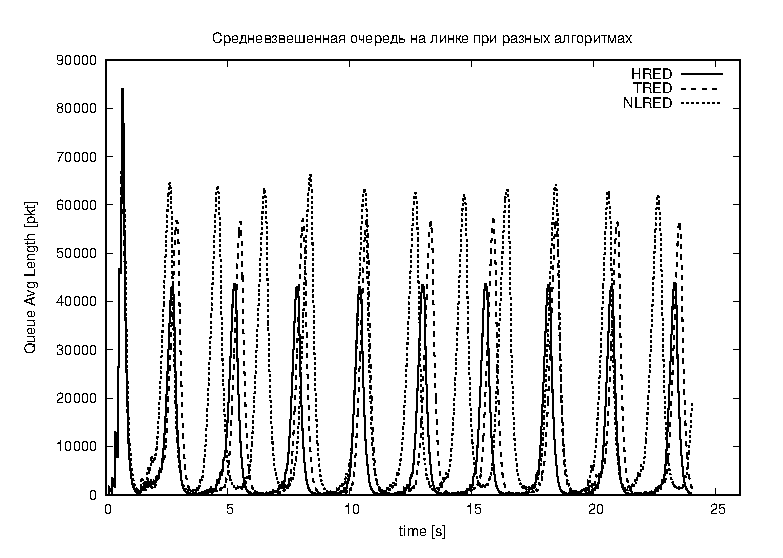
\includegraphics[width=0.7\linewidth]{image/av_queues_HTNl.eps}
  \caption{График средневзвешанной экспоненциальной очереди для HRED, TRED, NLRED}
  \label{fig:3.4}
\end{figure}

Расмматривая нелинейные модификации ~\ref{fig:3.4}, мы видим, что HRED наиболее подходящая модификация для сетей, где потеря пакетов не является значительной пролемой, а TRED показывает результаты, по значению средние с другими модификациями, увеличивает пропускную способность при
низкой нагрузке и уменьшает задержку при высокой нагрузке.  

Изучая адаптивные модификации ~\ref{fig:3.5},~\ref{fig:3.6}, ~\ref{fig:3.7}. Алгоритм Feng ARED показывает наименьшую амплитуду при достижении стационарного состояния. FARED и RARED имеют одинаковый алгоритм и отличаются только двумя коэфицентами, но RARED отбрасывает гораздо меньше пакетов. Powared показывает самую большую среднюю длину очереди и из вышеперчисленных показывет наибольший разброс между данными.


\begin{figure}[!ht]
  \centering
  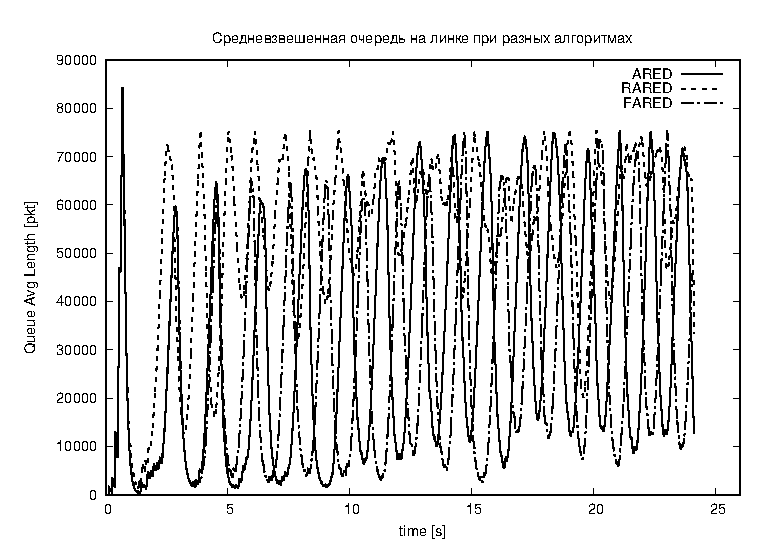
\includegraphics[width=0.7\linewidth]{image/av_queues_adaptive1.eps}
  \caption{График средневзвешанной экспоненциальной очереди для адаптивных алгоритмов}
  \label{fig:3.5}
\end{figure}

\begin{figure}[!ht]
  \centering
  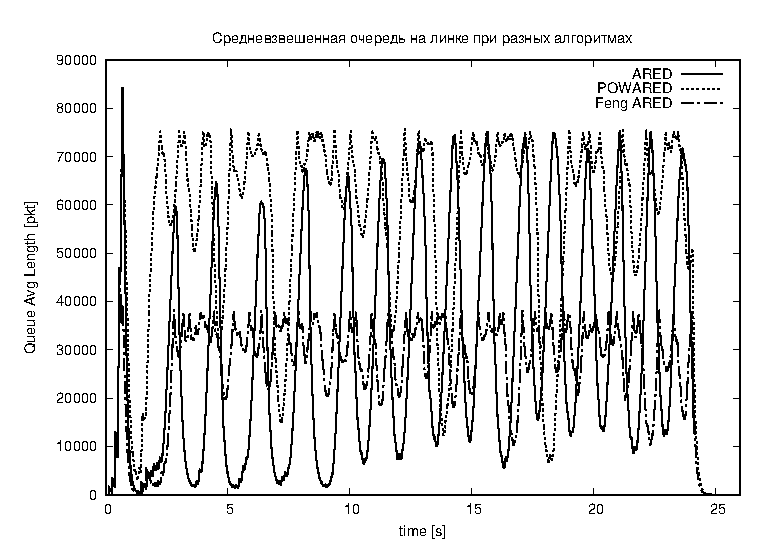
\includegraphics[width=0.7\linewidth]{image/av_queues_adaptive2.eps}
  \caption{График средневзвешанной экспоненциальной очереди для адаптивных алгоритмов}
  \label{fig:3.6}
\end{figure}

\begin{figure}[!ht]
  \centering
  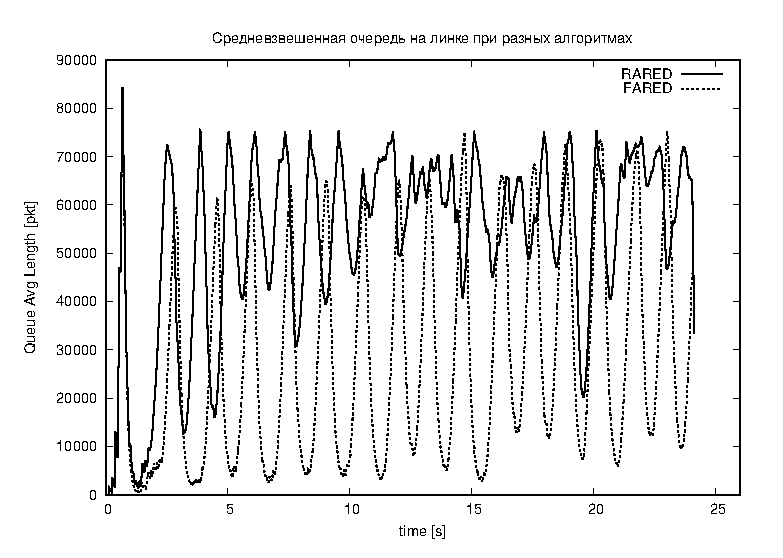
\includegraphics[width=0.7\linewidth]{image/av_queues_adaptive3.eps}
  \caption{График средневзвешанной экспоненциальной очереди для адаптивных алгоритмов}
  \label{fig:3.7}
\end{figure}













\chapter*{Заключение}
\addcontentsline{toc}{chapter}{Заключение}

За период практики в отделе технической поддержки пользователей
(департамент технологических и информационных ресурсов) РУДН и научных
центрах института прикладной математики и телекоммуникаций.  были
достигнуты все цели и решены все задачи, определенные в программе
научной практики направления подготовки 09.03.03 <<Прикладная
информатика>> программы <<Прикладная информатика>> (см. введение
отчёта по практике). В процессе прохождения практики я работал с
научной терминологией области исследований; научился собирать и
обрабатывать данные, необходимые для формирования
соответствующих выводов исследований; осуществлять целенаправленный
поиск информации на русском и английском языках о новейших научных
достижениях в Интернете и из других источников; строить и анализировать
имитационные модели обьекта исследований.

В результате прохождения данной практики я приобрел следующие
практические навыки, умения, универсальные и профессиональные
компетенции:

\begin{itemize}
\item способность управлять проектом на всех этапах его жизненного
  цикла (постановка задачи, планирование, реализация);
\item способность составлять естесвенно-научные отчеты с IMRAD
  структурой (введение, методы и материалы, результаты и дискуссия);
\item способность разрабатывать имитационные модели и проводить их
  анализ при решении задач в профессиональной области (составлена
  имитационная модель сети с алгоритмом управления очередью на 
  маршрутизаторе типа RED);
\item способность проведения работ по обработке и анализу
  научно-технической информации и результатов исследований (изучение
  необходимой литературы по теме исследования на русском и английском
  языках, подготовка литературного обзора по теме исследований).
\end{itemize}

Таким образом, в рамках практики я рассмотрел моделирование модуля RED
c помощью программного средства NS-2 версии 2.35. Также представлена
программная реализация имитационной модели сети модулем RED и проведен
сравнительный анализ результатов при моделировании сети с разными
входными параметрами, модификаций RED и типов TCP.




\renewcommand{\bibname}{Список литературы}
\cleardoublepage
\phantomsection
\addcontentsline{toc}{chapter}{Список литературы}
\bibliography{bib}

\bibliographystyle{ugost2008l} 
% \bibliographystyle{plain} 
% \bibliographystyle{gost2008l} 

\appendix

\chapter*{Приложения}
\addcontentsline{toc}{chapter}{Приложения}

Ссылка на репозиторий: 
\url{https://github.com/agsargsyan/study_2022-2023_practice}

\section*{Программа симуляции}

\begin{minted}[linenos,tabsize=2,breaklines]{bash}
- main.tcl
```
#Создать новый экземпляр объекта Symulator
set ns [new Simulator]

#Открыть трейс файл для nam, файл слишком большой, так что временно закомментируем
set nf [open output/out.nam w]
$ns namtrace-all $nf

#количество источников 
set N 20

#создание узлов
source "nodes.tcl"

#очередь		
source "queue.tcl"

#настройка времени моделирования  		
source "timing.tcl" 		

#визуализация
source "nam.tcl"   		

#процедура finish
source "finish.tcl"                                                                         

#Запуск программы
$ns run

 
```
- nodes.tcl
```
set node_(r0) [$ns node]  #первый маршрутизатор
set node_(r1) [$ns node]  #второй маршрутизатор	

for {set i 0} {$i < $N} {incr i} {
	set node_(s$i) [$ns node] 		#источник
	set node_(s[expr $N + $i]) [$ns node]	#приемник
	}

#линки между маршрутизаторами и другими узлами(размер буфера, время, тип очереди)
for {set i 0} {$i < $N} {incr i} {
	$ns duplex-link $node_(s$i) $node_(r0) 100Mb 20ms DropTail
	$ns duplex-link $node_(s[expr $N + $i]) $node_(r1) 100Mb 20ms DropTail
}

#линки между маршрутизаторами(размер буфера, время, тип очереди)
$ns simplex-link $node_(r0) $node_(r1) 20Mb 15ms RED
$ns simplex-link $node_(r1) $node_(r0) 15Mb 20ms DropTail

# Агенты и приложения:
for {set t 0} {$t < $N} {incr t} {
	$ns color $t green
	set tcp($t) [$ns create-connection TCP/Reno $node_(s$t) TCPSink $node_(s[expr $N + $t]) $t]
	$tcp($t) set window_ 32
	$tcp($t) set maxcwnd_ 32
	set ftp($t) [$tcp($t) attach-source FTP]
}

```

- nam.tcl
```
#визуализация цветов, формы, располажения узлов в nam
$node_(r0) color "red"
$node_(r1) color "red"
$node_(r0) label "RED"
$node_(r1) shape "square"
$node_(r0) label "square"

$ns simplex-link-op $node_(r0) $node_(r1) orient right
$ns simplex-link-op $node_(r1) $node_(r0) orient left
$ns simplex-link-op $node_(r0) $node_(r1) queuePos 0
$ns simplex-link-op $node_(r1) $node_(r0) queuePos 0

for {set m 0} {$m < $N} {incr m} {
	$ns duplex-link-op $node_(s$m) $node_(r0) orient right
	$ns duplex-link-op $node_(s[expr $N + $m]) $node_(r1) orient left 
}

for {set i 0} {$i < $N} {incr i} {
	$node_(s$i) color "blue"
	$node_(s$i) label "ftp"

}
```

- queue.tcl
```
#Лимит очереди
$ns queue-limit $node_(r0) $node_(r1) 300
$ns queue-limit $node_(r1) $node_(r0) 300


# Мониторинг размера окна TCP
set windowVsTime [open output/WvsT w]
set qmon [$ns monitor-queue $node_(r0) $node_(r1) [open output/qm.out w]]
[$ns link $node_(r0) $node_(r1)] queue-sample-timeout


# Формирование файла с данными о размере окна TCP
proc plotWindow {tcpSource file} {
   global ns
   set time 0.01
   set now [$ns now]
   set cwnd [$tcpSource set cwnd_]
   puts $file "$now $cwnd"
   $ns at [expr $now+$time] "plotWindow $tcpSource $file"
}

# Мониторинг очереди:
set redq [[$ns link $node_(r0) $node_(r1)] queue]
$redq set thresh_ 75
$redq set maxthresh_ 150
$redq set q_weight_ 0.002
$redq set linterm_ 10
$redq set drop-tail_ true

$redq set queue-in-bytes false
set tchan_ [open output/all.q w]
$redq trace curq_
$redq trace ave_
$redq attach $tchan_

#Для реализации разных модификаций RED,
$redq set gentle_ false 

#$redq set nonlinear_ 1
#$redq set hyperbola_ 1 
#$redq set quadratic_linear_ 1
#$redq set three_sections_ 1
#$redq set exponential_ 1
#$redq set smart_ 1
#$redq set double_slope_ 1

# Группа адаптивных алгоритмов
#$redq set adaptive_ 1
#$redq set feng_adaptive_ 1
#$redq set refined_adaptive_ 1
#$redq set fast_adaptive_ 1
#$redq set powared_ 1

```

- timing.tcl
```
#Задаем время симуляции
for {set r 0} {$r < $N} {incr r} {
        $ns at 0.0 "$ftp($r) start" 
        $ns at 1.0 "plotWindow $tcp($r) $windowVsTime"
        $ns at 24.0 "$ftp($r) stop"
}

$ns at 25.0 "finish"
```

- finish.tcl
```
#Finish procedure
proc finish {} {
   global ns nf
   $ns flush-trace
   close $nf
   global tchan_
   set awkCode {  
      {#запись данных в файлы очереди и средней очереди
         if ($1 == "Q" && NF>2) {
            print $2, $3 >> "output/temp.q";
            set end $2
         }
         else if ($1 == "a" && NF>2)
         print $2, $3 >> "output/temp.a";
      }
   }

   set f [open output/temp.queue w]
   puts $f "TitleText: RED"
   puts $f "Device: Postscript"

   if { [info exists tchan_] } {
      close $tchan_
   }
   #обновление данных
   exec rm -f output/temp.q output/temp.a
   exec touch output/temp.a output/temp.q

   exec awk $awkCode output/all.q

   puts $f \"queue
   exec cat output/temp.q >@ $f
   puts $f \n\"ave_queue
   exec cat output/temp.a >@ $f
   close $f
   # вывод в xgraph
   exec xgraph -bb -tk -x time -t "TCPRenoCWND" output/WvsT &
   exec xgraph -bb -tk -x time -y queue output/temp.queue &
   exit 0
}
\end{minted}
% \end{verbatim}


\section*{red.cc adaptive REDs}

\begin{minted}[linenos,tabsize=2,breaklines]{C++}

void REDQueue::updateMaxP(double new_ave, double now)
{
	double part = 0.4*(edp_.th_max - edp_.th_min);
	// AIMD rule to keep target Q~1/2(th_min+th_max)
	if ( new_ave < edp_.th_min + part && edv_.cur_max_p > edp_.bottom) {
		// we increase the average queue size, so decrease max_p
		edv_.cur_max_p = edv_.cur_max_p * edp_.beta;
		edv_.lastset = now;
	} else if (new_ave > edp_.th_max - part && edp_.top > edv_.cur_max_p ) {
		// we decrease the average queue size, so increase max_p
		double alpha = edp_.alpha;
                        if ( alpha > 0.25*edv_.cur_max_p )
			alpha = 0.25*edv_.cur_max_p;
		edv_.cur_max_p = edv_.cur_max_p + alpha;
		edv_.lastset = now;
	} 
}

void REDQueue::updateMaxP_refined_adaptive(double new_ave, double now)
{
  	double part = 0.48*(edp_.th_max - edp_.th_min);
 	if ( new_ave < edp_.th_min + part && edv_.cur_max_p > edp_.bottom) {
 		edv_.cur_max_p = edv_.cur_max_p * (1.0 - (0.17 * ((edp_.th_min + part) - new_ave) / ((edp_.th_min + part) - edp_.th_min))); 
 		edv_.lastset = now;
 		double maxp = edv_.cur_max_p;
 	} else if (new_ave > edp_.th_max - part && edp_.top > edv_.cur_max_p ) {
 		double alpha = edp_.alpha;
 		alpha = 0.25 * edv_.cur_max_p * ((new_ave - (edp_.th_max - part)) / (edp_.th_max - part));
 		edv_.cur_max_p = edv_.cur_max_p + alpha;
 		edv_.lastset = now;
 		double maxp = edv_.cur_max_p;
 	}
}


void REDQueue::updateMaxP_powared(double new_ave, double now)
{
  	double target = 0.5*(edp_.th_max + edp_.th_min);
  	int k = edp_.pwk;
  	int b = edp_.pwb;
  	int r = edp_.bf_size;
  	double v_ave = edv_.v_ave;
  	
  	
  	
  	double delta1 = abs(pow((v_ave - target)/(b * target), k));
  	double delta2 = abs(pow((target - v_ave)/(b * (r -target)), k));
 	
 	if ( new_ave < target && edv_.cur_max_p > edp_.bottom) {
 		edv_.cur_max_p = edv_.cur_max_p - delta1; 
 		edv_.lastset = now;
 		double maxp = edv_.cur_max_p; 
 	} else if (new_ave > target && edp_.top > edv_.cur_max_p ) {
 		edv_.cur_max_p = edv_.cur_max_p + delta2;
 		edv_.lastset = now;
 		double maxp = edv_.cur_max_p;
 	}
}

void REDQueue::updateMaxP_fast_adaptive(double new_ave, double now){
	  	double part = 0.48*(edp_.th_max - edp_.th_min);
		if ( new_ave < edp_.th_min + part && edv_.cur_max_p > edp_.bottom) {
 		edv_.cur_max_p = edv_.cur_max_p * (1.0 - (0.0385 * ((edp_.th_min + part) - new_ave) / ((edp_.th_min + part) - edp_.th_min))); 
 		edv_.lastset = now;
 		double maxp = edv_.cur_max_p;
 	} else if (new_ave > edp_.th_max - part && edp_.top > edv_.cur_max_p ) {
 		double alpha = edp_.alpha;
 		alpha = 0.0412 * edv_.cur_max_p * (new_ave - part) / part;
 		edv_.cur_max_p = edv_.cur_max_p + alpha;
 		edv_.lastset = now;
 		double maxp = edv_.cur_max_p;
 	}


}

\end{minted}

\section*{red.cc calculate drop probability}

\begin{minted}[linenos,tabsize=2,breaklines]{C++}
/*
 * Calculate the drop probability.
 */
double
REDQueue::calculate_p_new(double v_ave, double th_max, int gentle, double v_a, 
	double v_b, double v_c, double v_d, double max_p)
{	
	double target;
	double exponenta = 2.7182818285;
	double th_min = edp_.th_min;
	double p;
	if (gentle && v_ave >= th_max) {
		// p ranges from max_p to 1 as the average queue
		// size ranges from th_max to twice th_max 
		p = v_c * v_ave + v_d;
        } else if (!gentle && v_ave >= th_max) { 
                // OLD: p continues to range linearly above max_p as
                // the average queue size ranges above th_max.
                // NEW: p is set to 1.0 
                p = 1.0;
        } else if (edp_.quadratic_linear == 1) {
        	target = 2 * ((th_min + th_max)/3) - th_min;
        	if(v_ave < target){
        		p = 9 * max_p * ((v_ave-th_min)/(2*(th_max-2*th_min))) * ((v_ave-th_min)/(2*(th_max-2*th_min)));
        	} else if (v_ave >= target) {
        		p = max_p + 3*(1-max_p)*((v_ave-target)/(th_max+th_min));
        	}
        } else if (edp_.improved == 1) {
        	target = ((th_min + th_max)/3) + th_min;
        	if(v_ave < target){
        		p = 9 * max_p * ((v_ave-th_min)/(th_max + th_min)) * ((v_ave-th_min)/(th_max + th_min));
        	} else if (v_ave >= target) {
        		p = max_p + 3*(1-max_p)*(v_ave-target)/(2*(th_max - 2 * th_min));
        	}
        } else if (edp_.smart == 1) {
        	target = ((th_max - th_min)/2) + th_min;
        	if(v_ave < target){
        		p = max_p * pow(((v_ave-th_min)/(th_max - th_min)), 2);
        	} else if (v_ave >= target) {
        		p = max_p * pow(((v_ave-th_min)/(th_max - th_min)), 0.5);
        	}
        } else if (edp_.three_sections == 1){
        	double delta = (th_min+th_max/3);
        	if (v_ave < (th_min + delta)){
        		p = 9 * max_p * pow((v_ave-th_min)/(th_max-th_min), 3) ;
        		}
        	else if ((v_ave >= th_min + delta) && (v_ave < th_min + 2 * delta)){
        		p = max_p * (v_ave-th_min)/(th_max-th_min);
        		}
        	else if (v_ave >= th_min + 2* delta){
        		p =  9 * max_p * pow((v_ave-th_min)/(th_max-th_min), 3) + max_p;
        	} 
        }
        else if (edp_.double_slope == 1) {
        	double a = (2-2* edp_.omega)/(th_max - th_min);
        	double b = (2 * edp_.omega)/(th_max - th_min);
        	target = ((th_max + th_min)/2);
        	if(v_ave < target){
        		p = a * (v_ave-th_min);
        	} else if (v_ave >= target) {
        		p = 1 - edp_.omega + b * (v_ave - target);
        	}
        }
        else {
                // p ranges from 0 to max_p as the average queue
                // size ranges from th_min to th_max 
                p = v_a * v_ave + v_b;
                // p = (v_ave - th_min) / (th_max - th_min)
                
                /* Added by Mohit P. Tahiliani for Nonlinear RED (NLRED) - Start */
				if(edp_.nonlinear == 1){
					p *= p;		// This ensures probability is a quadratic function of "average queue size" as specified in NLRED Paper
				}
				else if (edp_.hyperbola == 1){
					p *= 1/p;	// This ensures probability is a hyperbola function of "average queue size" as specified in HRED Paper
				}
				else if (edp_.exponential == 1){ // Used for RED_e
					p = (pow(exponenta, v_ave)-pow(exponenta, th_min))/(pow(exponenta, th_max)-pow(exponenta, th_min));
				}
                p *= max_p; 
        }
	if (p > 1.0)
		p = 1.0;
	return p;
}
\end{minted}

\section*{red.h}

\begin{minted}[linenos,tabsize=2,breaklines]{C++}

	int feng_adaptive;	/* adaptive RED: Use the Feng et al. version */
	int refined_adaptive;	/* Added by Mohit P. Tahiliani for Refined Adaptive RED (Re-ARED) */
	int stabilized_adaptive;/* Added Stabillized Adaptive RED (SARED) */
	int nonlinear;		/* Added for Nonlinear RED (NLRED) */
	int hyperbola;		/* Added for Hyperbola RED (HRED)*/
	int quadratic_linear;   /* Added for Quadratic linear RED*/
	int three_sections;	/* Added for 3sections RED*/
	int exponential;	/* Added for exponential RED*/
	int improved;		/* Added for improved RED*/
	int smart;		/* Added for smart RED*/
	int modified;		/* Added for modified RED*/	 
\end{minted}

\section*{ns-default.tcl}

\begin{minted}[linenos,tabsize=2,breaklines]{C++}

/*Added for new RED alghorithms*/

Queue/RED set nonlinear_ 0
Queue/RED set hyperbola_ 0
Queue/RED set quadratic_linear_ 0
Queue/RED set three_sections_ 0
Queue/RED set exponential_ 0
Queue/RED set improved_ 0
Queue/RED set smart_ 0
Queue/RED set modified_ 0
\end{minted}


\section*{out.gp}

\begin{minted}[linenos,tabsize=2,breaklines]{C++}
#! /usr/bin/gnuplot -persist
set terminal postscript eps enhanced adobeglyphnames
set output "test.ps"
set encoding utf8

set xrange [0:26]

set terminal postscript eps
set output "av_queues_1GNl.eps"
set xlabel "Время [c]"
set ylabel "Длина очереди [пакеты]"
set title "Средневзвешенная очередь на линке при разных алгоритмах"
plot "classic.a" with lines linestyle 1 lt 1 lw 2 title "RED", "gentle.a" with lines linestyle 1 lt 2 lw 2 title "GRED", "nonlinear.a" with lines linestyle 1 lt 3 lw 2 title "NLRED" 

set terminal postscript eps
set output "av_queues_HTNl.eps"
set xlabel "Время [c]"
set ylabel "Длина очереди [пакеты]"
set title "Средневзвешенная очередь на линке при разных алгоритмах"
plot "hyperbola.a" with lines linestyle 1 lt 1 lw 2 title "HRED", "3.a" with lines linestyle 1 lt 2 lw 2 title "TRED", "nonlinear.a" with lines linestyle 1 lt 3 lw 2 title "NLRED" 
\end{minted}













\appendix
 %\newpage

\end{document}
